\documentclass{article}
\usepackage[utf8]{inputenc}
\usepackage{graphicx}
\usepackage{listings}
\usepackage{color}
\usepackage{enumitem}

\definecolor{dkgreen}{rgb}{0,0.6,0}
\definecolor{gray}{rgb}{0.5,0.5,0.5}
\definecolor{mauve}{rgb}{0.58,0,0.82}

\lstset{language=C,
  numbers=left,
  stepnumber=1,    
  firstnumber=1,
  numberfirstline=true
  aboveskip=5mm,
  belowskip=5mm,
  showstringspaces=false,
  columns=flexible,
  basicstyle={\small\ttfamily},
  numberstyle=\tiny\color{gray},
  keywordstyle=\color{blue},
  commentstyle=\color{dkgreen},
  stringstyle=\color{mauve},
  breaklines=true,
  breakatwhitespace=true
  tabsize=3
}

\title{Artificial Intelligence 1 \\ Lab 1}%Update the lab (assignment number)
\author{Name1 (student number 1) \& Name2 (student number 2) \\ Group name} %Change the names and fill in the student numbers and the group name (AI1/AI2/CS1 etc)
\date{day-month-year}%Update the date

\begin{document}

\maketitle

\section*{Theory}
\subsection*{Exercise 1}
%Your answers for the theoretical questions go here

\subsection*{Exercise 2}
%Your answers for the theoretical questions go here


\section*{Programming} 
%The programming part follows the same template used during ADinC and Imperative Programming
\subsection*{Program description}

The program asks for two numbers as inputs, and a search method, and looks for a way to produce the second number from the first, using the allowed operations and the given search method. It prints out the way of production, and the number of states enlisted and examined, if the program finds a solution within the given memory boundary.

\subsection*{Problem analysis}
There were several functions to implement: The BFS and DFS methods had to be improved to give a more efficient solution, the heap had to be filled to the skeleton of the method, and the IDS method had to written from skratch. Also, the program had to be extended to print the series of actions to the solution as well.  

\subsection*{Program design}
The design of the problems, in order of the questions is the following:
\begin{itemize}  
	\item In the BFS method, the task 0 to 100 runs out of memory, and in the DFS method the task 0 to 1 runs out of memory, the others in question 1 can be produced. The reason is, that the solutions are only checked when visited, and not when generated, so the DFS only checks in the sequence of the last action (rightmost branch), and the BFS adds 1 level of depth to the complexity, that can be avoided. The solution is to check for goals when generating a node, and not only when visiting them. To implement this, we defined a helper function newValue that can be used to calculate the new values for every action iteratively, and also allows to check for solutions iteratively before enlisting the new node. Thus, a loop for node generation is implemented within the search functions, that loops through the "cases", the valid operations.
	\item To keep track of the preceding actions in every node generated, we defined a new struct called Operation, that stores an operatoin applied to a state, and the value after that. We also extended the struct State with an array of operations, and we add all the operations in the sequence here. When a solution is found, we add the last operation, and simply print out the sequence that is stored in the State's operation array (called path).
	\item For implementing the heap, we modified the heap functions from Algorithms and Data Structures to take a fringe as an argument. This way, the fringe's array could be used for a heap. We also modified the relations to store the minimum in the beginning. The heap functions are added to the fringe files. The heap order is based on the cost of the paths, as it is suggested in the fifth question. With the heap functions added, we only had to add enqueue and dequeue to the fringe functions. This gives and optimal path of steps 6 and cost 9 between 0 and 42.
	\\
	\\
	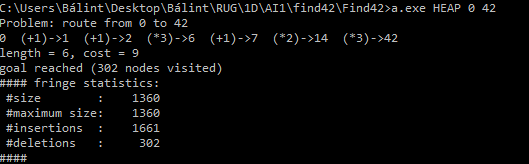
\includegraphics{optimalpath.png}
	\item The iterative deepening is basically a limited DFS with increasing limits, and the limited DFS is basically a DFS with a given limit. To use these properties, we did not implement the IDS in the fringe, but rather in the search function: we added an extra loop, that is only repeated when the mode is IDS, and an other if statement before generating nodes, that checks if the depth is within limit (that is always true in the other modes, since the limit in those is practically set to infinity). The extra loop increases the limit by 1 in every iteration, and runs it as a DFS, with the limit checker.
	\item Comparing the different methods, the following conclusions can be drown:
	\begin{itemize}
		\item The DFS method uses relatively small memory, but it only examines the leftmost branch of the tree, and the children that are generated on that branch. Thus, in many cases, when the children is not accesible on that branch it reaches the memory limit without finding the solution, so it is not an optimal solution. However, if the solution is on that branch, DFS finds it the quickest. The memory complexity is O(6m) for 6 = branching factor and m = maximal depth, but with no limits it can be arbitrarily large. The time complexity is also O(6m), since it never returns from any states with no limits or constraints. Note that m is practically infinite, giving a high chance of extending the memory limit.
		\item The BFS method enqueues all the generated nodes, and calculates upon the oldest one, so it proceeds horizontally on the tree. This means, that it stores all the nodes on a depth level, giving high memory usage, and high time complexity (no ordering in this case), but is reliable in finding the solution. This gives us the time comlexity of $O(6^d)$, with branching factor 6 and the solution depth d. The memory complexity is also $O(6^d)$.
		\item The HEAP method works similarily as the BFS, but it uses ordering based on the cost, that is not neccessarily helps with finding the solution earlier, so it does not reduce time or memory complexity, but ensures, that the given answer is cost-optimal. The complexities here depend on the optimal path cost C*, giving complexities $O(6^{1 + C*})$, where the minimal cost is 1.
		\item The IDS method runs int the order of the BFS, but inherits the low memory usage of DFS. The time complexity is the same order as in BFS, but in practice it is slightly higher, since many nodes are generated multiple times. However, the memory complexity is low, only in O(bd). If the task is to find a way, and not to find the optimal way, this is the most reliable, and most memory-efficient search method in this task. 
	\end{itemize} 
\end{itemize}
\subsection*{Program evaluation}
The program runs with no memory leaks. The complexity of the solution depends on which search method was used, as listed in the last point in the previous section.

\subsection*{Program output}
The program outputs a sequence of operations starting from the first number to produce the second number. The outputs may differ using different modes, since most of the times there are multiple solutions, and the modes visit the nodes in different order. Only the heap method is optimal in the sense of giving the lowest cost path. The program also outputs the fringe statistics, making it simple to compare the methods.

\subsection*{Program files}
%copy code files into listings using the \begin{listing} command as follows:
\subsubsection*{search.c}
\lstinputlisting{search.c}
\subsubsection*{fringe.c}
\lstinputlisting{fringe.c}
\subsubsection*{fringe.h}
\lstinputlisting{fringe.h}


\end{document}